\documentclass{article}
\usepackage{floatrow}
\usepackage{graphicx}
%\usepackage{subfig}
\usepackage[label font=bf,labelformat=simple]{subfig}% <-- changed
\floatsetup[figure]{style=plain,subcapbesideposition=top}

\begin{document}
	\begin{figure}[htb]
		\centering
		\sidesubfloat[]{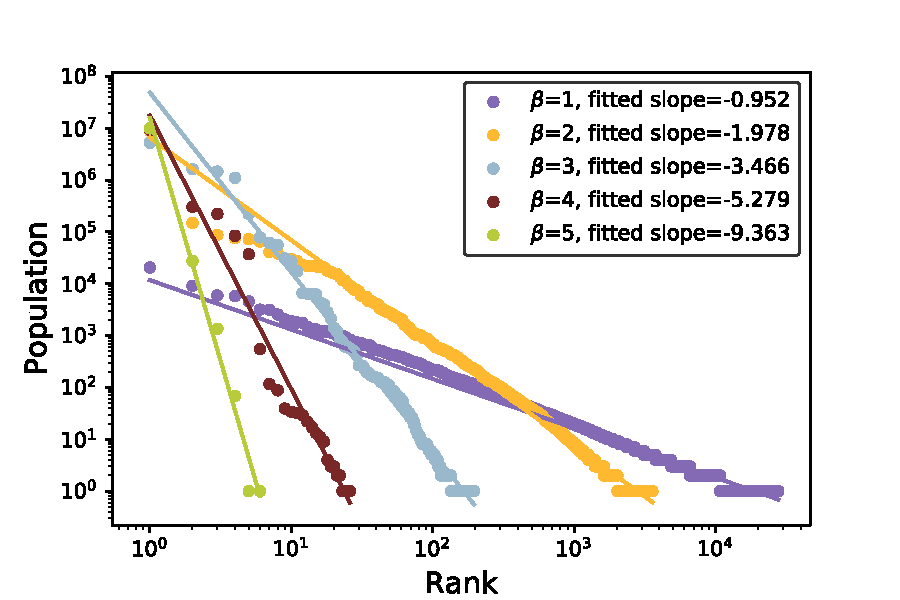
\includegraphics[width=.3\textwidth]{pics/zipf.pdf}\label{fig:a}}
		\hfil
		\sidesubfloat[]{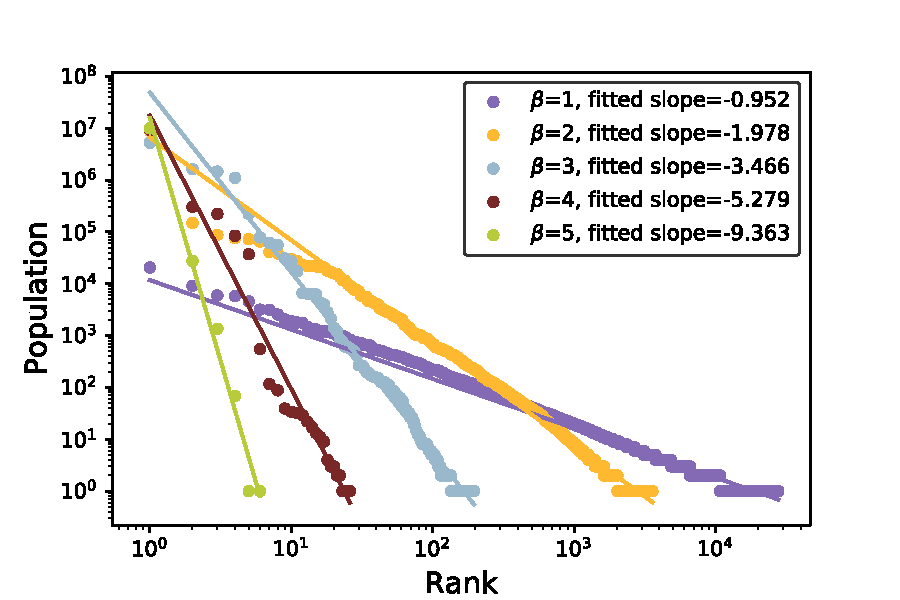
\includegraphics[width=.3\textwidth]{pics/zipf.pdf}\label{fig:b}}
		\caption{\textbf{(a)} The distribution of population among cities. In the simulation we take $N^* = 10^5$ and alternate $\beta$s. The realistic Zipf's coefficient is reproduced when $\beta\approx 1$. The theoretical predictions of the slopes are $-\beta$, and is well approximated when $\beta$s are small. Larger $\beta$ reduce the chance of latter city's emergence. Thus the spatial aspects of the SYM strengthen inequality. This result confirms that Zipf's law is valid for growing urban systems where all cities share the same rate to grow. From the other master equation we analyze that this observation vanishes if total growing force is finite. \textbf{(b)} The population distribution as a function of distance from a district's center. The vertical axis is logarithmic processed, which represents the exponential decaying of population distribution. Regardless of the finite-sample effect, we fit the middle part of spatial population density to the exponential distribution with a slope of $-1.076$.}
		\label{fig:myfigure}
	\end{figure}
	Figure \ref{fig:myfigure} consist three sub figures: \ref{fig:a} and \ref{fig:b}
\end{document}